\documentclass[a4paper, 11pt]{article}


\usepackage{amsmath}
\usepackage[cmintegrals]{newtxmath}
\usepackage{bm}
\usepackage{cite}
\usepackage{algorithmic}
\usepackage{graphicx}
\usepackage{xcolor}
\usepackage{url}
\usepackage{epigraph}
\usepackage{caption}
\usepackage{threeparttable}
\usepackage{siunitx}
\usepackage[margin=1.1in]{geometry}
\usepackage{wrapfig}

\begin{document}


\title{Swipe Without Age and Gender - An Ionic Application}
\author{
Aden Kenny - 300334300
}
\date{August 31, 2018}
\maketitle



\section{Architectural Design}

\begin{wrapfigure}{r}{0.5\textwidth}
\centering
\captionsetup{format=hang}
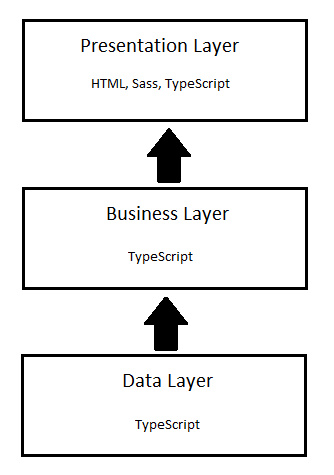
\includegraphics{arch.png}
\caption{A diagram of the application architecture}
\end{wrapfigure}

Our applications uses a fairly standard three tier architecture. It has a presentation layer of HTML, Sass, and a little bit of TypeScript, a business layer of TypeScript, and finally a data layer of TypeScript. There is a strict communication protocol between the three different layers. The data layer can only interact with the business layer, the presentation layer can only interact with the business layer, and the business layer can interact with both the data layer and the business layer. This means that all interactions with external components must go through an intermediary (the business layer) before interacting with the with the user (the presentation layer).

~\\
The presentation layer is seen and interacted with by the users. This layer handles all user interaction, and the users should only ever see this layer. HTML is used to create the structure of the user interface and therefore the presentation layer. Sass is then used to style the HTML, and there is a small amount of TypeScript used for the interface (booleans for Angular ngIf, etc.). It communicates only with the presentation layer. When communicating with the presentation layer it either sends information about options the user has selected or actions they have carried out. When receiving data from the business layer, the data is related to options or queries the user has made, and this data is then used to update the view the user sees and provide interactivity between the user and the app.

~\\
The business layer acts as a sort of middleman between the presentation and data layers. The business layer exists exclusively of TypeScript code with functions to parse data from the data layer, functions to update the presentation layer, and functions to modify the local state of the system. All interaction between the presentation layer and data layer must go through the business layer. The overall design means that when the user performs an action such as viewing another users profile, a message will be sent from the presentation layer to the data layer. The business layer will then update, and send a message to the presentation layer to update with some sort of loading behaviour, and a message is then sent to the data layer to fetch the required data to fully update the presentation layer. This data from the data layer is then sent to the business layer where it is parsed for use, and then finally a message is sent to the presentation layer to update to the final state required for the user action.

~\\
The data layer sends data to and from the external Firebase services (see the Firebase Integration section below). When fetching data, a message is sent from the business layer to the data layer telling it to fetch data from the external services, this data is then sent to the business layer. The reverse of this scenario is taken when sending data to the external services.

~\\
Our architecture in reality matches up pretty well with the three-tier model. The presentation and business layers are made up by the files that make up each page, and the data layer is made up by our two service classes that are injected into our first page. The presentation layer and business layer are fairly loosely coupled especially since there is no direct DOM manipulation in our code. The data and business layers are extremely loosely coupled, and the data layer could quite easily be swapped out with another with no adverse consequences.


\section{Firebase Integration}
Our application is a Tinder clone, therefore needed a significant amount of external interaction. We choose to use Firebase for our external storage as it is fairly easily to interact with, and there is good documentation available online. 

~\\
As our service is account based, the first service we used from Firebase was the authentication service \cite{FirebaseAuth}. This was fairly easy to set up, and it handles all user authentication, from account creation, to logging in. The Firebase authentication service means that users can securely create an account, and their data is safely salted and hashed server side.

~\\
In our application each user has a profile picture, and in order to display this profile picture to other users the picture had to be stored server side. In order to solve this problem we used Firebase Storage. This allowed us to create a folder for each user where their profile picture is saved. When a user views the profile of another user, the profile picture of the second user is downloaded from our Firebase Storage.

~\\
Finally, we used Firebase's Realtime Database \cite{firebaseDB} to store user details, including personal information, and also to store conversations. Getting user details is fairly similar to profile pictures as mentioned above, but since the user data is all text, we can store it in a standard database rather than a specialised file storage solution. Conversations are also stored as text in the database, and both users have one conversation object. This means there are no concurrency issues, and there is a single source of truth without having server-side code.

~\\
In order to integrate our Firebase services into our app, we made authentication and database services that are injected into our Home page, and a reference to them can be gotten by any pages that need them through static getters. All database and authentication actions are in the data layer and are therefore separate and uncoupled from the business and presentation layers.

~\\
I found Firebase simple and pleasant to use, and the only gripe I had with it was the fact that it only supports a NoSQL database. NoSQL is useful in situations where you need to scale your database when you have large amounts reads and writes as the database can be distributed over ordinary, cheap servers. In the case of our app, there isn’t much risk of the database needing to be scaled so a relational database probably would have been better for our needs. Additionally, the non-relational structure of a NoSQL database did not provide much of an advantage to us as our user data was fairly structured and uniform.

\section{UX decisions} 
\subsection{Color Scheme}

We have employed a warm colour scheme for our user interface (see Figure 1 for a screenshot of the home page). We chose this colour palette as warm colours can have a major impact on how a user interacts with a user interface. Warm colours are ``associated with passion, energy, impulsiveness, happiness, coziness, and comfort.” \cite{color}. There are two focuses we tried to draw from a warm colour palette, the passionate and impulsive side, and the happy and comforting side. The passionate, energetic size was considered to be extremely important as these are key things in a Tinderlike dating app. If a user feels energetic and passionate, they are much likely to use the app and make connections with other people. Additionally, if a user feels more impulsive they are more likely to sign up for the app, or to swipe right on people, and this means that the energetic feel that a warm colour scheme brings helps to persuade a potential user to use our app.

\begin{wrapfigure}{r}{0.5\textwidth}
\centering
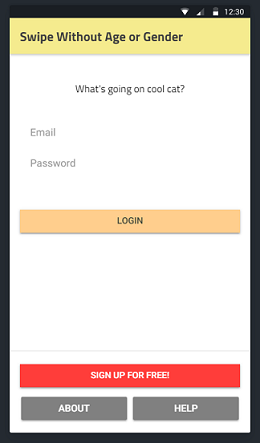
\includegraphics{WarmColours.png}
\caption{A screenshot of the Home page}
\end{wrapfigure}

~\\
The happy and comforting nature of the warm colour palette was also considered to be extremely important to the overall feel of our app. Meeting and talking new people can be very stressful process and we want our users to feel as comfortable as possible. 

~\\
Our primary colour is a pale yellow colour which can be seen in Figure 1, on the navigation bar. This yellow is present on all screens (through the nav bar) and it helps to produce a warming effect that evokes pleasant feelings \cite{color}. The pale yellow nav bar is then complemented by a peach-orange colour that is present on most non-call to action buttons in our app. This colour is halfway between yellow and orange and helps to provide a warming effect to buttons that are meant to be pleasant to the user and have pleasant results. Examples of this include the button that takes the user to the cruise screen, the "login" button (see Figure 1), and the "message hub" button. 

~\\
Additionally, our call to action buttons (see the sign up button in Figure 1) are a vibrant candy red that draws the users eye and encourages them to the action, and they fit in our warm colour scheme by providing a sense of "energy and confidence" \cite{color}.

\subsubsection{Alternative Color Scheme}

~\\
Figure 2 shows an alternate colour scheme that was considered. It is a much cooler palette, with blues and purples being the dominant colours. Cool colours are said to be ``often associated with calm, trust, and professionalism." \cite{color}. An overall cool colour palette would have then delivered an overall image of competency and professionalism. We considered the warm colour palette's energy, coziness and the comfort it inspires in users to be more important the aforementioned benefits of the proposed cool colour scheme. This is because we favoured a warm, playful, and happy feel for the app and we considered that be important in a dating app. A cool colour palette would suit an app that targets a more professional background such as LinkedIn.

\begin{figure}
\centering
\begin{minipage}{.55\textwidth}
  \centering
  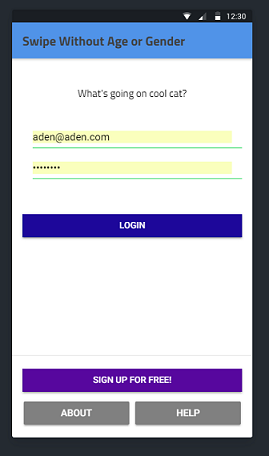
\includegraphics[width=.7\linewidth]{coolcolor.png}
  \captionof{figure}{A screenshot of the Home page showing the alternate, cool colour palette}
  \label{fig:test1}
\end{minipage}%
\begin{minipage}{.55\textwidth}
  \centering
\captionsetup{format=hang}
  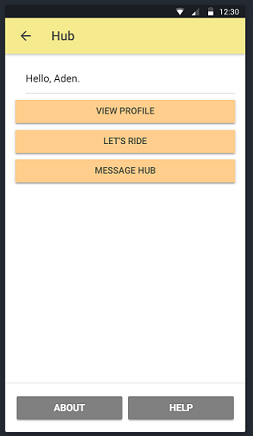
\includegraphics[width=.7\linewidth]{grouping.png}
  \caption{A screenshot of the Hub page}
  \label{fig:test2}
\end{minipage}
\end{figure}

\subsection{Law of Common Region}
We kept the law of common region \cite{commonRegion} in mind when designing our user interface. The law of common region states that ``Elements tend to be perceived into groups if they are sharing an area with a clearly defined boundary." \cite{commonRegion}, and we have taken into account this phenomenon. Items which are related, such as groups of buttons, are grouped together in common region and share common features (size, colour). A good example of this can be seen in Figure 3 where two distinct groups can be noticed. Firstly we have the grouping of the three warmly coloured buttons in the upper centre of the screen. These buttons provide the user with options to go to the main functionality of the app. These buttons are seen as grouped together due to being in the same area, and due to the sharing common features such as colour and size.

~\\
There is another clear grouping at the bottom of the screen in Figure 3. The two buttons in the footer are used to access pages that provide more information to the user about the app. These buttons are grouped together both by the extremely clear sharing of area (the footer), and by having a common colour and size (grey and 45\% of the width of the page respectively).

~\\
These two clear groupings show that elements being together are strongly perceived as groups as they share a clearly defined boundary and share common features, in this case size and colour. This is a clear example of the law of common region in practice, and we kept this in mind when designing our interface by making sure that items that we wanted to be perceived as a group were together and similar to each other.  

\begin{wrapfigure}{r}{0.5\textwidth}

\centering
\captionsetup{format=hang}
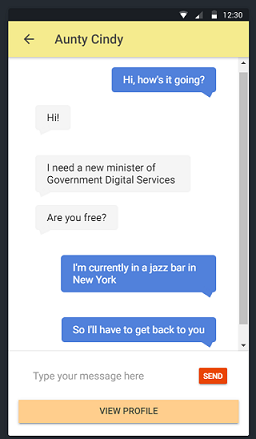
\includegraphics{choices.png}
\caption{A screenshot of the Conversation page}
\end{wrapfigure}
\subsection{Hick's Law}
Hick's Law states that ``the time it takes to make a decision increases with the number and complexity of choices." \cite{hicks}. We took this into account when designing user interface. The main idea behind Hick's Law is that the time it takes a user to do something or make a decision will increase with the amount of options that a user has. In our app we tried to reduce the number of options a user has available to them at any time. Less choices means the user will spend less time contemplating each of them, and they will move onto a choice quicker, which is ideal for our app.

~\\
An excellent example of this in our app is the conversation page. This is the page a user is taken to after they have matched with another user and want to chat to them. The user has only three options on this page. The first is option is to click the back button at the top to be taken back to the conversation hub, the second option is to view the other users profile, and finally the third option is to type and send a message to the other user. This is a very small collection of possible user options, especially when compared to other messaging apps such as Messenger or WhatsApp where the user is presented with a myriad of options. Less options, as per Hick's Law, means that users will spend less time trying to make choices are more time interacting with our app. We kept this purposely in mind, cutting out options we considered to be unnecessary all through out the app, and this resulted in a focused app where the user doesn't have too many options which means they should be able to use the app faster and get on with other things that are far more important in their lives.

\subsubsection{Hick's Law, Again}

An alternative design decision that we considered was making the app more complex, as in adding more choices for the user. This is illustrated when considering the initial design document, it stated that the app would have more messaging functionality (sending of pictures and other multimedia), but we saw the complexity more options adds, as per Hick's Law. Other examples of options that were considered that could have made the app more complex include splitting up of functionality in multiple pages and elements, and a settings menu. Ultimately we decided against most of these options as we felt they added needless complexity that would have made it harder to use our app.
\section{Ionic Critique}
The most appropriate thing to compare Ionic with would probably be native development (Android and IOS). The main differences surround the tools used to develop the app. In the case of Ionic we use HTML, Sass, and TypeScript. This is in direct contrast to Android where the entire app is generally written in Java (there are other options such as Kotlin) with a bit of XML. Ionic provides a sort of separation of concerns due to this three part split. A major downside of this three part structure is having to work with more tools which in turn adds more complexity. 

~\\
The structure of the user interface of an Ionic app is implemented in HTML, then styling is applied to this with Sass (inline styling with HTML is possible). Finally, any more complex behaviour, or interaction with other pages is done with TypeScript code. This provides a fairly separate hierarchy of design which is split into three layers. 

~\\
The use of HTML is a both a strength and weakness of Ionic. It allows for rapid development, as the creation of an interface purely with HTML is very fast, especially when compared with native mobile development, where both the structure and styling are made with the same tool (Java or Swift). Another major strength of using HTML is that it is familiar to many developers already.
Obviously HTML has some long standing issues that are well known such as being quite verbose, and not particularly suited for human reading (some of the same issues as XML has). 

~\\
My biggest problem with Ionic is the use of Sass as a styling tool. Rather than having styling built into the structure of the user interface, Sass is used for styling. Sass is a superset of CSS which means it inherits many of CSS's warts, even if it fixes many of CSS's problems (introducing variables). There are multiple right ways to do anything with CSS which means when asking how to do something, you will get multiple different answers all with their own pros and cons. Some things are far harder than they should be in CSS, such as centering \cite{cssCenter}, especially when compared to Android where an element can be centered easily with a layout such as RelativeLayout. CSS and by extension Sass development is full of “hacky” workarounds especially when trying to style Ionic components \cite{toastStyle}. 

~\\
TypeScript is probably the best part of the Ionic development process, especially when compared to normal web development with JavaScript. TypeScript is strict superset of JavaScript that adds static typing, which shifts an entire class of runtime bugs to compile time bugs, allowing easier debugging by catching bugs earlier. TypeScript’s static typing also allows for easier reasoning about the code as the whole system feels less like a “house of cards”, and more stable. The static type system also allows for better autocompletion and refactoring support.


\section{Appendices}
\subsection{Division of Work}
For this project I worked in a pair with Simon Pope (3003343009). The app idea and architecture are a joint work, and then we divided the pages between us and then worked on them separately.

\subsubsection{Joint Work}
\begin{itemize}
	\item{Architectural Design}
	\item{Data services (entire data layer)}
\end{itemize}

\subsubsection{Aden}

\begin{itemize}
	\item{About Page}
	\item{Conversation Page}
	\item{Help Page}
	\item{Home Page}
	\item{Loading Page}
	\item{Message Hub Page}
	\item{Register Page}
\end{itemize}

\subsubsection{Simon}

\begin{itemize}
	\item{Cruise Page}
	\item{Edit Details Page}
	\item{Hub Page}
	\item{Match Page}
	\item{Post Review Page}
	\item{Review Page}
	\item{View Match Page}
	\item{View Profile Page}
\end{itemize}

\bibliographystyle{ieeetr}

\bibliography{bibliography}
\end{document}